\section{Revisão Sistemática}

\begin{frame}		
	\begin{block}{Revisão Sistemática}
		A revisão da literatura iniciou com um estudo exploratório seguido de uma resivão sistemática. Dessa forma, foi possível: 
		\begin{enumerate}
			\item Encontrar o estado da arte na área de recomendação de atividades em \emph{workflows} científicos.
			\item Compreender o problema;
			\item Encontrar termos específicos da área;
			\item Definir palavras-chave;
		\end{enumerate}
	\end{block}
\end{frame}

%\begin{frame}		
%	\begin{block}{Planejamento}
%		Para definir as palavras-chave foi usada a metodologia PICO, que após ser aplicada, retornou os resultados:
%		\begin{enumerate}
%			\item \textbf{Population:} \emph{scientific}, \emph{workflow} e \emph{pipeline};
%			\item \textbf{Intervention:} \emph{recommendation}, \emph{provenance}, \emph{suggestion}, \emph{forecast}, \emph{advice}, \emph{design}, \emph{visualization}, \emph{recommender}, \emph{construct}, \emph{proposal}, \emph{guidance}, \emph{counsel}, \emph{composition}, \emph{activity}, \emph{shimming}, \emph{inference}, \emph{reuse}, \emph{reusing}, \emph{semiautomatically}, \emph{similarity}, \emph{match}, \emph{matching}, \emph{complete}, \emph{auto};
%			\item \textbf{Control:} O alvo da pesquisa são as técnicas usadas;
%			\item \textbf{Output:} O alvo da pesquisa é descobrir como são validadas as técnicas propostas.
%		\end{enumerate}			
%	\end{block}
%\end{frame}
%
%\begin{frame}		
%	\begin{block}{Planejamento}
%		Após definir os quatro grupos, foi especificada a seguinte \emph{string} de busca:
%		
%		``(\emph{scientific} \textbf{and} (\emph{workflow} \textbf{or} \emph{pipeline})) \textbf{and} (\emph{recommendation} \textbf{or} \emph{provenance} \textbf{or} \emph{suggestion} \textbf{or} \emph{forecast} \textbf{or} \emph{advice} \textbf{or} \emph{design} \textbf{or} \emph{visualization} \textbf{or} \emph{recommender} \textbf{or} \emph{construct} \textbf{or} \emph{proposal} \textbf{or} \emph{guidance} \textbf{or} \emph{counsel} \textbf{or} \emph{composition} \textbf{or} \emph{activity} \textbf{or} \emph{shimming} \textbf{or} \emph{inference} \textbf{or} \emph{reuse} \textbf{or} \emph{reusing} \textbf{or} \emph{semiautomatically} \textbf{or} \emph{similarity} \textbf{or} \emph{match} \textbf{or} \emph{matching} \textbf{or} \emph{complete} \textbf{or} \emph{auto})''.
%	\end{block}
%\end{frame}

\begin{frame}		
	\begin{block}{Condução}
		\begin{figure}
			\tiny
			\begin{minipage}[b]{0.46\textwidth}
				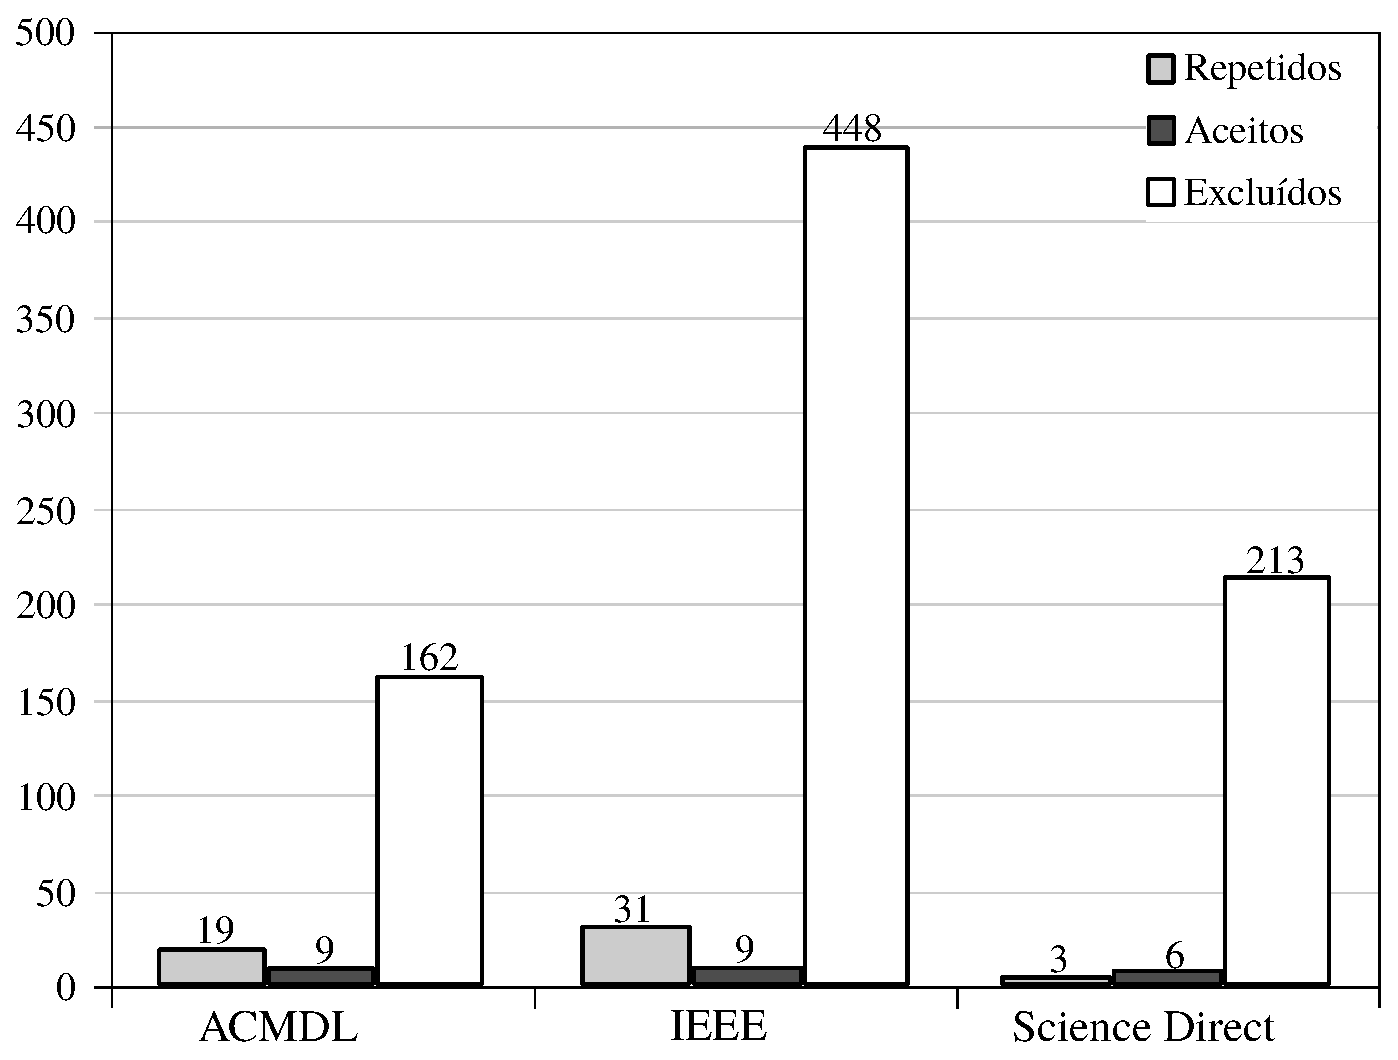
\includegraphics[width=\textwidth]{./secoes/RevisaoDaLiteratura/GraficoQuantidade.eps}
				\caption{Quantidade de artigos por técnica}
			\end{minipage}
			%\qquad
		     \hspace{0.1cm}
			\begin{minipage}[b]{0.46\textwidth}
				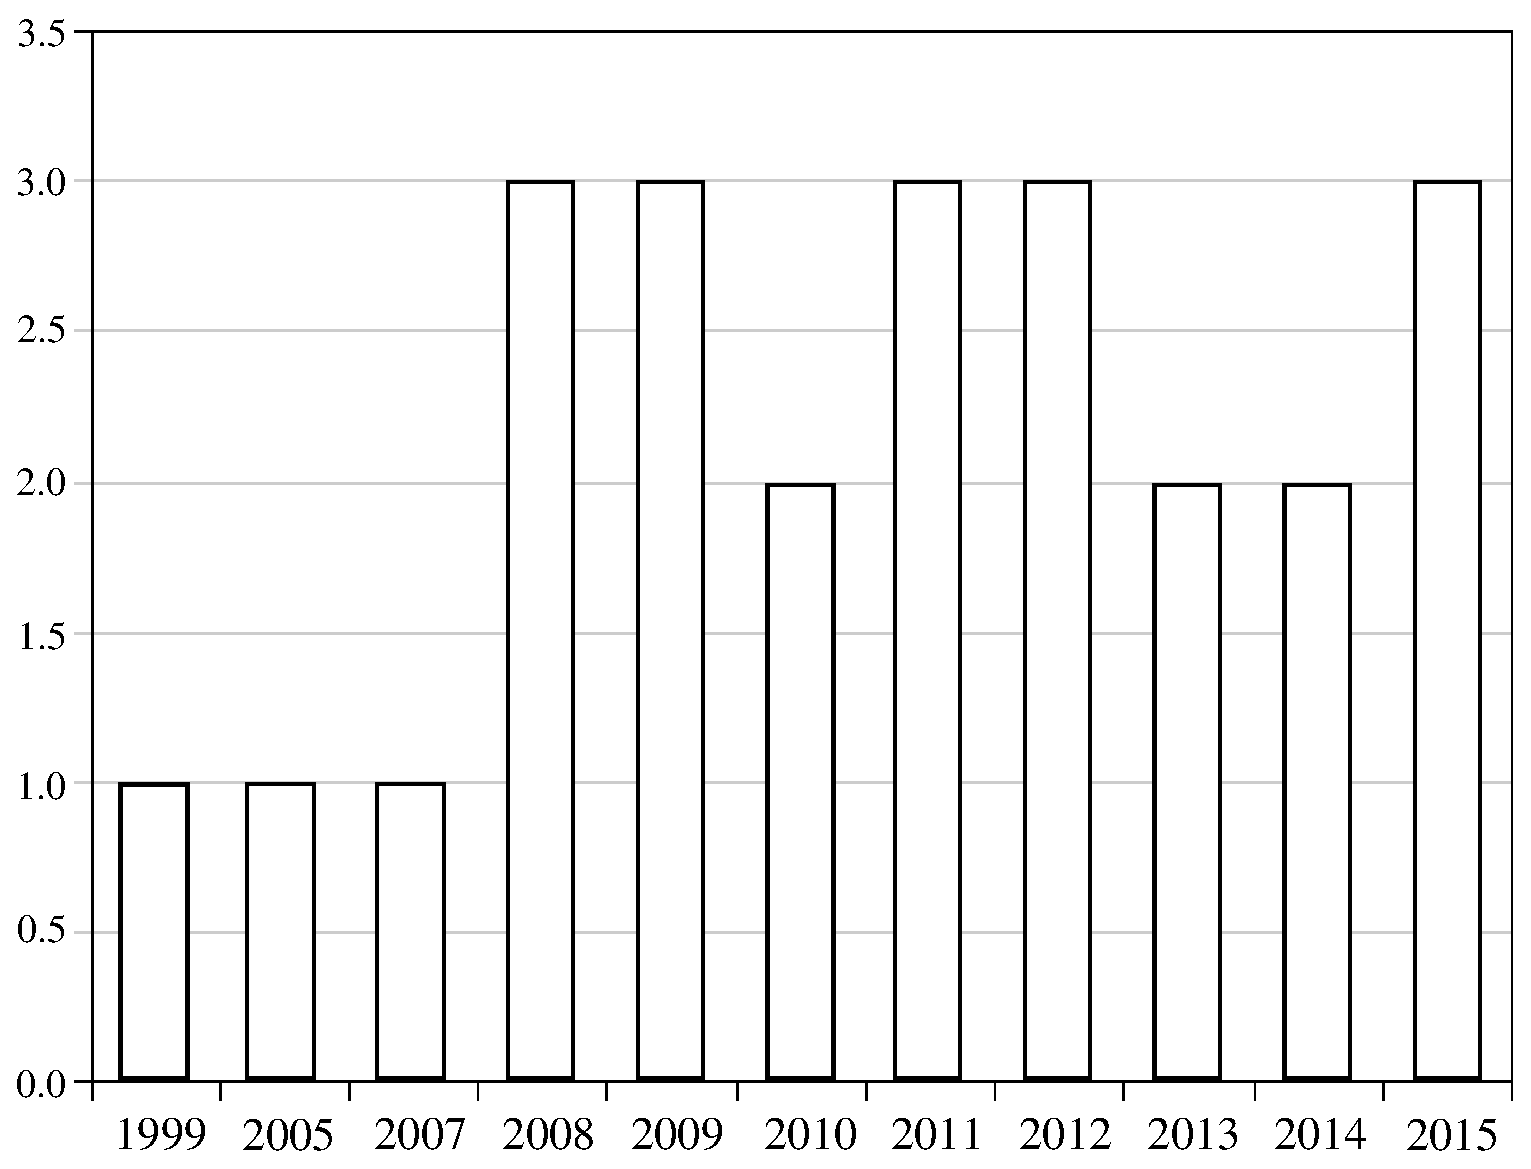
\includegraphics[width=\textwidth]{./secoes/RevisaoDaLiteratura/GraficoQuantidadeAno.eps}
				\caption{Artigos por ano de publicação}
			\end{minipage}
		\end{figure}
		
	\end{block}
\end{frame}

\begin{frame}		
	\begin{block}{Execução}
		Observa-se que a técnica de proveniência é a mais usada seguida por: i) Frequência; ii) Entrada e saída; iii) Itemsets; e iv) Ontologias.
		\begin{figure}
			\begin{minipage}[b]{0.6\textwidth}
				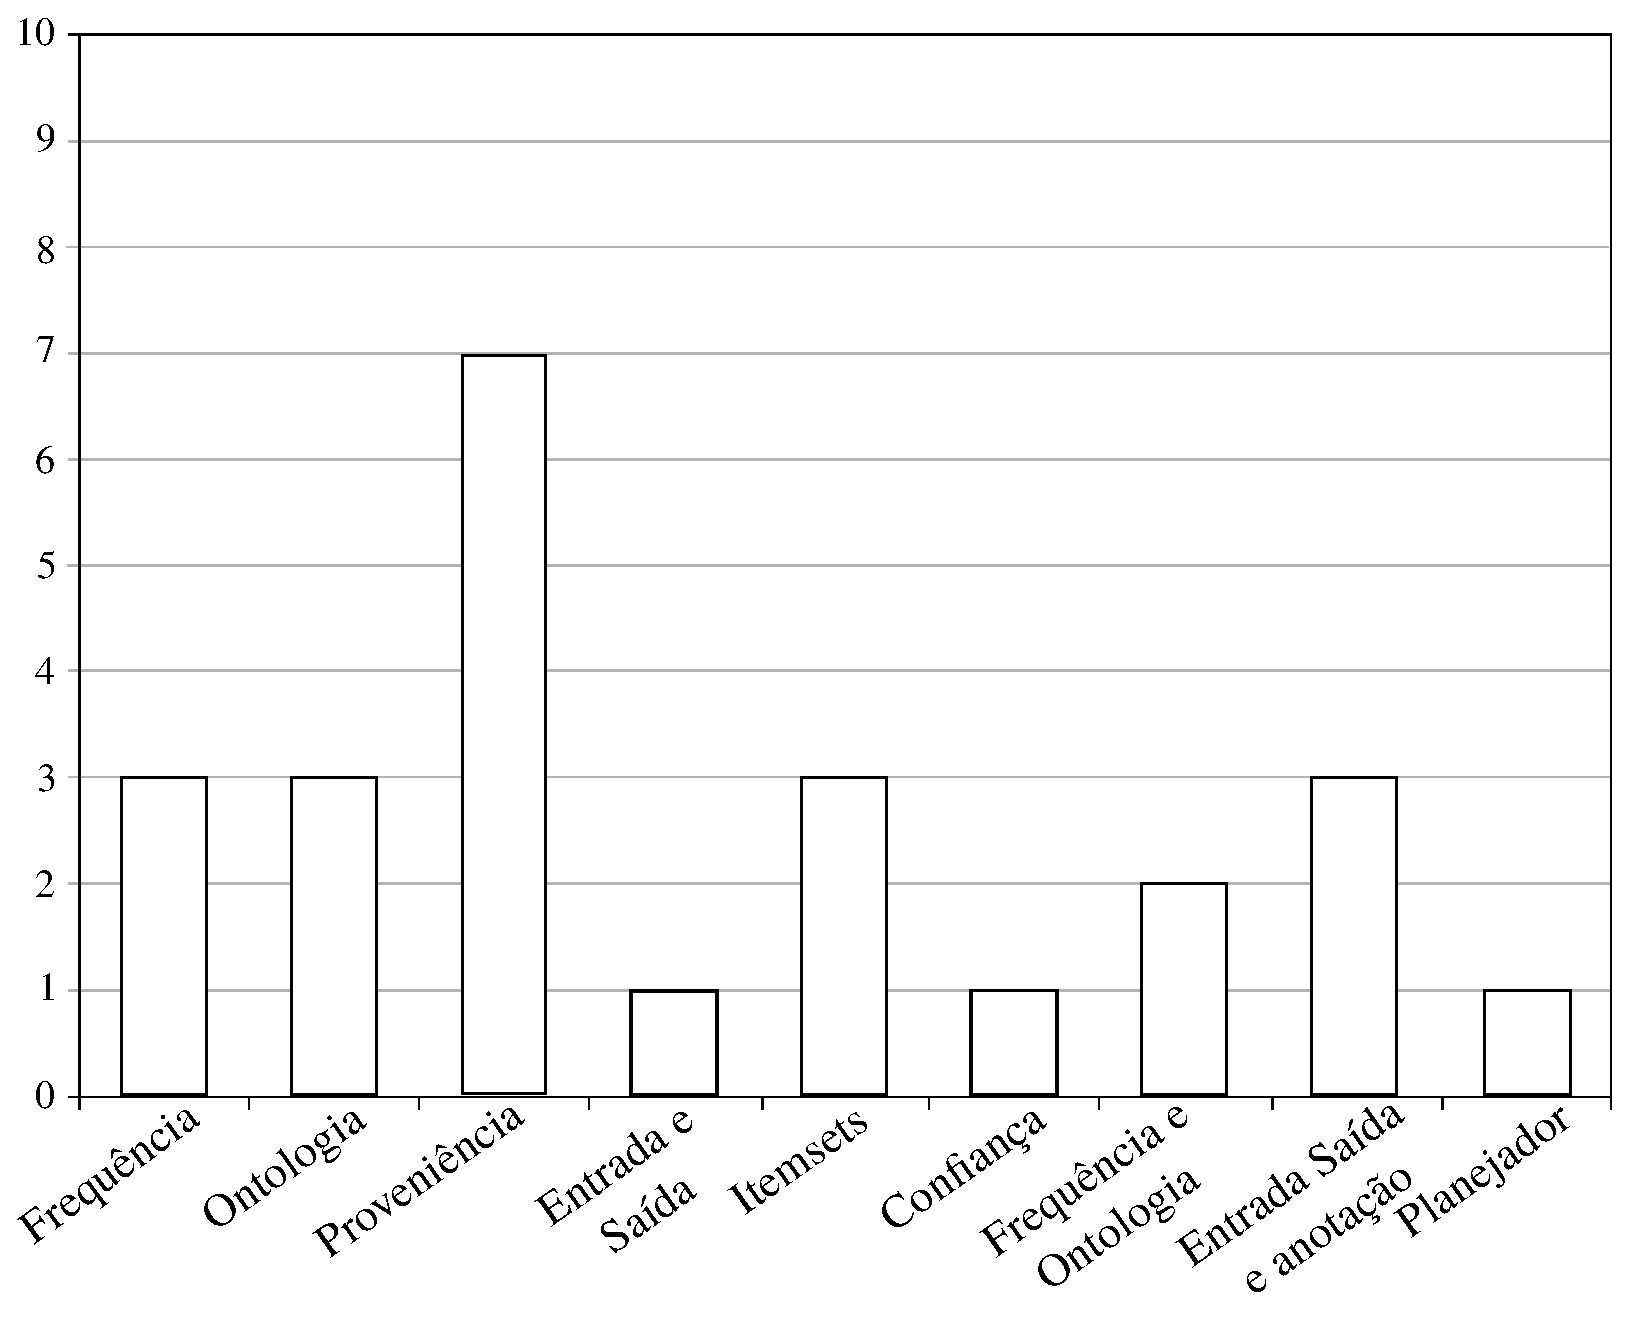
\includegraphics[width=\textwidth]{./secoes/RevisaoDaLiteratura/GraficoQuantidadeTecnica.eps}
				\caption{Quantidade de artigos por técnica}
			\end{minipage}
		\end{figure}
		
	\end{block}
\end{frame}

\begin{frame}		
	\begin{block}{Comparação da técnica proposta com as da literatura correlata}
		As principais vantagens da técnica proposta, em relação as da literatura correlata, são considerar as dependências de entrada e saída, semântica e a frequência de atividades. 
		
		Além disso, não há requesito de dados de proveniência, rede social, confiança entre usuários ou tipo de atividade: i) Shim; ii) Simples; e/ou iii) Subworkflow.
	\end{block}
\end{frame}

